\begin{figure}[t]
\centering
\begin{minipage}[t]{0.1429\textwidth}
\centering \colorbox{white}{\textbf{\scalebox{.8}{G. truth}}}
\end{minipage}\begin{minipage}[t]{0.1429\textwidth}
\centering \colorbox{white}{\textbf{\scalebox{.8}{Standard}}}
\end{minipage}\begin{minipage}[t]{0.1429\textwidth}
\centering \colorbox{white}{\textbf{\scalebox{.8}{AR (ours)}}}
\end{minipage}\begin{minipage}[t]{0.1429\textwidth}
\centering \colorbox{white}{\textbf{\scalebox{.8}{Standard}}}
\end{minipage}\begin{minipage}[t]{0.1428\textwidth}
\centering \colorbox{white}{\textbf{\scalebox{.8}{AR (ours)}}}
\end{minipage}\begin{minipage}[t]{0.1429\textwidth}
\centering \colorbox{white}{\textbf{\scalebox{.8}{Standard}}}
\end{minipage}\begin{minipage}[t]{0.1429\textwidth}
\centering \colorbox{white}{\textbf{\scalebox{.8}{AR (ours)}}}
\end{minipage}\vspace{-0.4\baselineskip}

\begin{minipage}{0.1429\textwidth}
\centering\textbf{ }
\end{minipage}\begin{minipage}[t]{0.1429\textwidth}
\centering \scalebox{0.65}{Pix.}
\end{minipage}\begin{minipage}[t]{0.1429\textwidth}
\centering \scalebox{0.65}{Pix.}
\end{minipage}\begin{minipage}[t]{0.1429\textwidth}
\centering \scalebox{0.65}{Pix., Feat.}
\end{minipage}\begin{minipage}[t]{0.1428\textwidth}
\centering \scalebox{0.65}{Pix., Feat.}
\end{minipage}\begin{minipage}[t]{0.1429\textwidth}
\centering \scalebox{0.65}{Pix., Feat., GAN}
\end{minipage}\begin{minipage}[t]{0.1429\textwidth}
\centering \scalebox{0.65}{Pix., Feat., GAN}
\end{minipage}

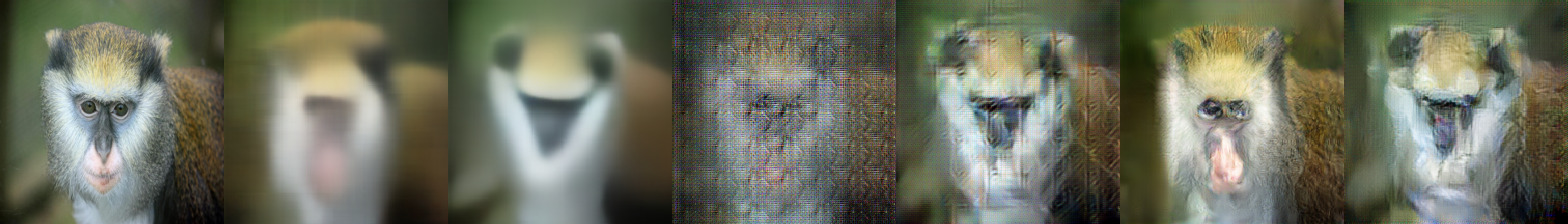
\includegraphics[width=\textwidth]{figs/ablation/ablation_tile2.jpg}

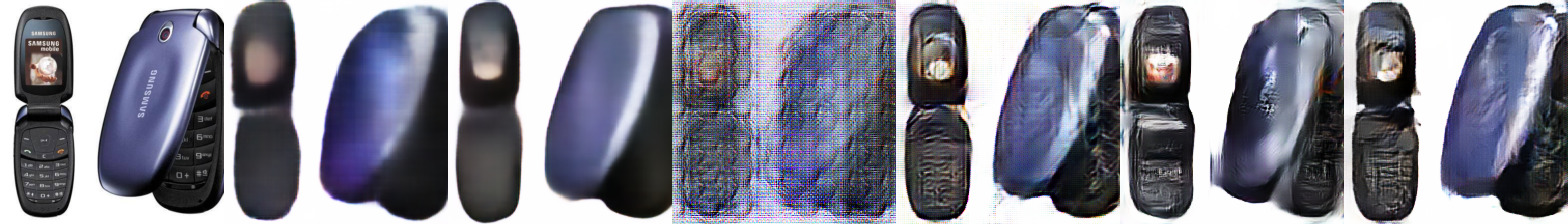
\includegraphics[width=\textwidth]{figs/ablation/ablation_tile9.jpg}

\caption{\label{fig:inversion_alexnet}AlexNet feature inversion on ImageNet. \layer{Conv5} features are inverted using our proposed generator under three different training criteria. Reconstructions from AR features are more faithful to the ground-truth image.}
\vspace{-0.4cm}
\end{figure}
